% options:
% thesis=B bachelor's thesis
% thesis=M master's thesis
% czech thesis in Czech language
% english thesis in English language

\documentclass[thesis=B,czech]{FITthesis}[2011/06/14]

\usepackage[utf8]{inputenc} % LaTeX source encoded as UTF-8

\usepackage{graphicx} %graphics files inclusion
% \usepackage{amsmath} %advanced maths
% \usepackage{amssymb} %additional math symbols

% % list of acronyms
% \usepackage[acronym,nonumberlist,toc,numberedsection=autolabel]{glossaries}
% \iflanguage{czech}{\renewcommand*{\acronymname}{Seznam pou{\v z}it{\' y}ch zkratek}}{}
% \makeglossaries

\newcommand{\tg}{\mathop{\mathrm{tg}}} %cesky tangens
\newcommand{\cotg}{\mathop{\mathrm{cotg}}} %cesky cotangens

% % % % % % % % % % % % % % % % % % % % % % % % % % % % % % 
% ODTUD DAL VSE ZMENTE
% % % % % % % % % % % % % % % % % % % % % % % % % % % % % % 

\department{Katedra softwarového inženýrství}
\title{Systém pro daňovou evidenci krátkodobých akcí skautských organizací}
\author{František Hána} %jméno autora bez akademických titulů
\authorWithDegrees{František Hána} %jméno autora včetně akademických titulů
\supervisor{Mgr. Petr Matyáš}
\acknowledgements{Doplňte, máte-li komu a za co děkovat. V~opačném případě úplně odstraňte tento příkaz.}
\abstractCS{V~několika větách shrňte obsah a přínos této práce v~češtině. Po přečtení abstraktu by se čtenář měl mít čtenář dost informací pro rozhodnutí, zda chce Vaši práci číst.}
\abstractEN{Sem doplňte ekvivalent abstraktu Vaší práce v~angličtině.}
\placeForDeclarationOfAuthenticity{V~Praze}
\keywordsCS{Nahraďte seznamem klíčových slov v češtině oddělených čárkou.}
\keywordsEN{Nahraďte seznamem klíčových slov v angličtině oddělených čárkou.}

\begin{document}

% \newacronym{CVUT}{{\v C}VUT}{{\v C}esk{\' e} vysok{\' e} u{\v c}en{\' i} technick{\' e} v Praze}
% \newacronym{FIT}{FIT}{Fakulta informa{\v c}n{\' i}ch technologi{\' i}}

\begin{introduction}
	%sem napište úvod Vaší práce
\end{introduction}

\chapter{Analýza a návrh}
\section{Srovnání jiných systémů}
Nenašel jsem žádný skautský online systém, který by byl používán více středisky. Většina středisek buď žádný online systém nepoužívá nebo mají systém, který si sami naprogramovali.
\subsection{Systém střediska Hiawatha Praha}
Systém je zakomponovaný do webových stránek střediska (\url{https://www.hiawatha.cz/}). Přihlášeným uživatelům umožnuje zakládat, upravovat a mazat akce. U každé akce můžeme přidat předběžný rozpočet. Po realizaci akce můžeme přidat i čerpané částky z jednotlivých kategorií a vyplnit seznam účastníků. Vedoucí může akci odevzdat, čímž umožní editaci pouze hospodáři střediska.
Výhody systému:
\begin{itemize}
	\item možnost sestavit rozpočet i výsledovku
	\item možnost přidat k akci reportáž a fotoalbum
	\item možnost předání akce hospodáři
	\item možnost přidat seznam účastníků
	\item počítá počet účastníků v jednotlivých kategoriích
\end{itemize}
Nevýhody systému:
\begin{itemize}
	\item minimální možnost nastavení uživatelských práv
	\item není propojen se systémem SkautIS
	\item částky v jednotlivých kategoriích, se musí spočítat mimo systém
	\item není možné evidovat paragony
	\item není možné zadat osobu mimo nabízený seznam
\end{itemize}


\subsection{Systém střediska Blaník}
Středisko Blaník využívá vlastní systém naprogramovaný v php skládající se ze tří základních částí. První část LTOI (\url{http://lab.blanik.info/ltoi/}) - Letní tábor a obnova inventáře - slouží pro vyúčtování táborů. Zadávají se zde odděleně informace o táboře, příjmy, výdaje, účastníci a cestovní příkazy. Veškeré informace je možné nechat vyexportovat do formátu csv nebo rtf.

Druhá část nazvaná INV (\url{http://lab.blanik.info/inv/}) slouží k inventarizaci majetku jednotlivých oddílů. Pokud jsme v části LTOI nastavili výdaj s příznakem \uv{inv}, tak ho nyní můžeme jednoduše importovat do této části. Získáme zde také přehled zda na majetek byla čerpána dotace, jeho pořizovací a aktuální hodnotu a informaci o jeho vyřazení.

Třetí a zároveň nejnovější (leden 2012) částí sytému je ROP (Roční oddílová pokladna). Zde se účtují pokladny jednotlivých oddílů za celý rok. 

Výhody systému:
\begin{itemize}
	\item možnost nastavit počet dnů účasti u jednotlivých účastníků táborav (LTOI)
	\item automatická kontrola vnitřních vztahů mezi účastníky a příjmy (LTOI)
	\item propojení části LTOI s částí INV 
	\item dobrý přehled o majetku oddílu (INV)
	\item možnost exportovat do dále upravitelné podoby (csv, rtf)
	\item možnost vyplnit cestovní příkaz (LTOI)
	\item možnost předat vyučtování akce hospodáři (LTOI)
\end{itemize}
Nevýhody systému:
\begin{itemize}
	\item malý počet účetních kategorií (LTOI)
	\item není propojen se systémem SkautIS
	\item veškeré věci jsou napevno zadané v kódu - včetně ceny benzínu apod.
	\item možnost upravovat i údaje, které jsou stálé - IČO střediska
	\item nulová podpora napovídání jmen účastníků
	\item uživatelsky nepřívětivé přidávání řádků
	\item nutnost zadávat vše textově místo použití standartních html značek (radio button pro označení řádku ke smazání)
	\item nejednotnost ovládání v jednotlivých částech 
\end{itemize}


\section{Specifikace požadavků}
\subsection{Funkční požadavky}
\begin{itemize}
	\item umí založit novou akci
	\item umí uzavřít akci
	\item umí evidovat akce minulé
	\item umí přijmout údaje z paragonu a ty pak spravovat
	\item umí rozdělit paragony do kategorií a spočítat jejich sumu
	\item umí udělat seznam účastníků
	\item umí udělat hromadný příjmový doklad
	\item umí kontrolovat přístupová práva
	\item umí spravovat účastníky na akcích
	\item design stránky není předmětem závěrečné práce
\end{itemize}

\subsection{Nefunkční požadavky}
\begin{itemize}
	\item webová aplikace v jazyce PHP
	\item aplikace komunikuje se systémem SkautIS přes web services
	\item aplikace má české uživatelské rozhraní
	\item aplikace funguje na PHP 5 $\geq$ 5.2.0, Mysql 5
\end{itemize}

\section{Uživatelské role}
Uživatelské role vycházejí z uživatelských rolí ze systému SkautIS. V systému rozlišuji, jestli je přihlášen jako \uv{člen} v dané jednotce či jako její \uv{vedoucí/administrátor}.
TODO

\section{Akce}
\label{sec:eventDescription}
Každá akce má parametry
\begin{itemize}
	\item ID\_Event
	\item pořadatel (povinný)
	\item název (povinný) 
	\item začátek (povinný)
	\item konec (povinný)
	\item typ (výprava, seminář, ...)
	\item rozsah (oddílová, středisková, ... )
	\item místo konání
	\item vedoucí akce (povinný)
	\item zástupce vedoucího akce
	\item hospodář akce
\end{itemize}
kde pořadatel, název, začátek, konec, typ a rozsah jsou povinné pro založení akce a před uzavřením akce musí být vyplněn i vedoucí akce. ID\_Event je identifikátor přidělený systémem SkautIS při založení akce.

\subsection{Životní cyklus akce}
 \begin{figure}[h] \centering
 	\includegraphics[width=0.7\textwidth]{img/state-diagram.jpg}
 	\caption[Životní cyklus akce]{Životní cyklus akce}\label{fig:state-diagram}
 \end{figure}
 Životní cyklus akce vychází z možností entity Event ze systému SkautIS. Ta může nabývat tyto stavy:
 
 \begin{itemize}
 	\item rozpracována
	\item uzavřena
	\item zrušena
 \end{itemize} 
 
Akce je ve stavu \uv{rozpracována} hned po jejím vytvoření a to dokud akci neuzavřeme nebo nezrušíme.

U \uv{uzavřené} akce je evidováno kdy a kdo ji uzavřel a v případě potřeby ji lze znovu otevřít do stavu \uv{rozpracována} a dále upravovat.

Změna stavu akce na \uv{zrušená} je nevratný krok a po té už akce bude přístupná pouze pro čtení nebo úplné vymazání ze systému.

\section{Případy užití}
\begin{figure}[h]\centering
 	\includegraphics[width=0.7\textwidth]{img/use-case.jpg}
 	\caption[Případy užití]{Use case diagramy}\label{fig:use-case}
\end{figure}
Vedoucí může založit akci, u které musí vyplnit povinné údaje (viz \ref{sec:eventDescription}) a pokud chce tak může i volitelné.

Může později změnit údaje, zadané při vytváření akce, pokud je akce rozpracována. 

Lze do seznamu účastníků přidávat osoby z vybrané jednotky, vytvořit nového účastníka i odebírat účastníky. U účastníků dále lze nastavit počet dní strávených na akci a výši účastnického poplatku. 

V pokladní knize lze evidovat všechny příjmy a výdaje akce, roztříděné do jednotlivých kategorií. Jednotlivé položky lze upravovat, mazat nebo exportovat.

Pokud máme akci hotovou, můžeme ji označit jako uzavřená a tím zamezit její editaci bez toho, aby ji někdo znovu otevřel.

\section{Výběr technologií}
\subsection{PHP}
Na poli PHP frameworků je v současné době hned několik velkých hráčů. Mezi nejznámější patří Symfony, Zend Framework a Nette Framework.

Symfony obsahuje velmi silný databázový framework Doctrine, ale nemá českou komunitu.

Zend Framework vyvíjí firma Zend Technologies Ltd., která stojí za jádrem PHP od verze 4. Mezi hlavní výhody Zend Frameworku patří velké množství již napsaných komponent, silné zázemí komunity a Zend Technologies Ltd. Naopak mu je často vytýkána špatná práce s formuláři a příliš dlouhé názvy, které snižují přehlednost kódu. 

Nette Framework, vyvíjený Nette Foundation, se v posledních letech prosazuje na české scéně čím dál tím více. Jeho hlavními přednostmi jsou jednoduchá práce s formuláři, šablonovací systém Latte a početná komunita. Často však bývá kritizován za to, že jeho vývoj je řízen jeho zakladatelem Davidem Grudlem a nikoli komunitou.

Já jsem si zvolil Nette Framework pro jeho dobré zpracování v oblasti formulářů a protože s ním již několik let pracuji. Důležitým faktorem při rozhodování byl i směr dalšího vývoje frameworku. Protože s jeho směřováním souhlasím, bude v budoucnu možné aplikaci dále rozšiřovat. Konkrétně jsem si vybral verzi pro PHP 5.2 bez prefixů.

\subsubsection*{Nette Framework}\label{netteDescription}
Pro tvorbu aplikací v Nette Framework se používá softwarová architektura Model-View-Controller (MVC). MVC slouží k oddělení kódu zajištujícího aplikační logiku (model) od kódu zajištujícího obsluhu (controller) a od způsobu výsledného zobrazení(view).

\begin{quotation}
Model je datový a zejména funkční základ celé aplikace. Je v něm obsažena aplikační logika. Jakákoliv akce uživatele (přihlášení, vložení zboží do košíku, změna hodnoty v databázi) představuje akci modelu. Model si spravuje svůj vnitřní stav a ven nabízí pevně dané rozhraní. Voláním funkcí tohoto rozhraní můžeme zjišťovat či měnit jeho stav.
\cite{netteModel}
\end{quotation}

V Nette Frameworku byl pojem controller nahrazen pojmem \uv{presenter}. Presentery obsluhují požadavky, získávají data od modelu a předávají je v potřebné podobě do daného view, které zajistí jejich zobrazení.

View jsou zde řešeny šablonovacím systémem Latte (\url{http://doc.nette.org/cs/templating#toc-latte}), který zajištuje ochranu proti XSS \cite{xss}, možnost použít makra a mnoho dalšího.

\subsection{Databáze}
Databázi jsem vybral MySQL, protože je dostupná na většině hostingů a pro rozsah projektu postačuje. Pro práci přístup k databázi jsem měl na výběr mezi využitím základní MySQL funkcí zabudovaných v PHP a použitím některé PHP knihovny pro práci s databází. Použití základních funkcí PHP jsem zavrhl, protože je velmi těžké udržet v kódu přehlednost a práce s připojením je velmi nekomfortní.

Doctrine 2 je jedna z nejznámějších knihoven pro práci s databází využívajících ORM, avšak na některá volání potřebuje příliš SQL dotazů.

NotORM, od Jakuba Vrány, se prezentuje jako plnohodnotná alternativa k běžným ORM a prezentuje se svojí rychlostí oproti ostatním \cite{notorm}. NotORM jsem již v minulosti vyzkoušel, ale práce s ním mi nevyhovovala. 

Nette Framework přímo nabízí vlastní vrstvu pro práci s databází \url{http://doc.nette.org/cs/database}. Vychází z NotORM, ale má trochu odlišnou syntaxi. Mě nevyhovuje ze stejných důvodů jako NotORM.

David Grudl kromě Nette Frameworku vytvořil také databázovou vrstvu dibi \url{http://dibiphp.com/}. Já jsem si ji velmi oblíbil pro její jednoduchost a protože mi nediktuje přesný způsob použití. Vybral jsem si ji pro tento projekt, protože podle mého názoru plnohodnotně pokryje databázové potřeby projektu a práci s ní dobře znám a vyhovuje mi.

Pro přístup do databáze přes Dibi máme dvě možnosti. Buď přes objekt DibiConnection, kterému v konstruktoru předáme parametry spojení a pak na něm budeme volat jednotlivé dotazy. Nebo přes statický objekt dibi, který je po prvním nastavení dostupný kdekoliv a stačí volat dotazy bez dalšího nastavování.

\begin{figure}[h]\centering
\begin{verbatim}

$params = array(
    'driver'   => 'mysql',
    'host'     => 'localhost',
    'username' => 'uzivatelske_jmeno',
    'password' => 'heslo',
    'database' => 'nazev_databaze',
);

//1. možnost - přístup skrz objekt
$db = new DibiConnection($params);
$db->query('SQL dotaz');

//2. možnost - statický přístup
dibi::connect($params); //stačí nastavit pouze jednou
dibi::query('SQL dotaz');

\end{verbatim}
\caption{ukázka použití Dibi}
\end{figure}

\subsection{Frontend}
HTML kód na výstupu bude generován ze šablonovacího systému Nette Frameworku s využitím maker Latte, které jsou také součástí. Hlavními výhodami Latte maker jsou automatické escapování a přehlednost napsaného kódu. Zde je ukázka z dokumentace \url{http://doc.nette.org/cs/templating#toc-latte} pro ilustraci čitelnosti kódu s Latte makry. 
\begin{figure}[h]
\caption{ukázka použití Latte - vypsání seznamu položek}
\begin{verbatim}
//bez použití Latte
<?php if ($items): ?>
    <?php $counter = 1 ?>
    <ul>
    <?php foreach ($items as $item): ?>
        <li id="item-<?php echo $counter++ ?>"><?php
        echo htmlSpecialChars(mb_convert_case($item, MB_CASE_TITLE)) ?>
        </li>
    <?php endforeach ?>
    </ul>
<?php endif?>

//zapsané pomocí Latte
<ul n:if="$items">
    <li n:foreach="$items as $item" id="item-{$iterator->counter}">
    {$item|capitalize}</li>
</ul>
\end{verbatim}
\end{figure}

Pro formátování HTML výstupu a některé Java Scriptové komponenty použiji \uv{Twitter Bootstrap}, což je mladý projekt od vývojářů z firmy Twitter. Více informací najdeme na \url{http://twitter.github.com/bootstrap/}. Ostatní Java Scriptové komponenty a události budou využívat populární knihovnu \uv{JQuery}, o které najdeme informace na \url{http://jquery.com/}.

\section{Datový model}
\begin{figure}[h] \centering
 	\caption[Doménový model]{Doménový model}\label{fig:domain-model}
	\includegraphics[width=1\textwidth]{img/domain-model.png}
\end{figure}
Datový model se v průběhu psaní aplikace velice zmenšil, díky několika novým verzím SkautISu, během kterých přibyl typ akce \uv{obecná akce} s možností přiřazení účastníků. V mojí databázi tedy budu uchovávat paragony a jejich kategorie. 
Tabulka \uv{chits} uchovává všechny paragony a je navázána přes \uv{actionId} na konkretní akci ve SkautISu a přes \uv{category} na tabulku \uv{chitsCategory}. Dále obsahuje 
 \begin{itemize}
 	\item datum přijetí paragonu do pokladní knihy
 	\item jméno příjemce
 	\item účel výplaty
 	\item částku
	\item způsob výpočtu částky - např. 10*17+13
	\item příznak jestli byl paragon smazán
\end{itemize} 

Tabulka \uv{chitsCategory} 
 \begin{itemize}
 	\item název kategorie
 	\item zkratku kategorie
 	\item jestli je doklad příjmový nebo výdajový
 	\item parametr pro řazení kategorií
 	\item příznak jestli byla kategorie smazána 
\end{itemize}
Každá akce i s účastníky je v systému SkautIS navázána na konkretní jednotku. A paragony jsou k dané akci navázány podle \uv{ID\_Event} dané akce. 

\section{Navigace}
 \begin{figure}[h] \centering
 	\includegraphics[width=1\textwidth]{img/navigation.png}
 	\caption[Navigační model]{Navigační model vytvořený ve Web Ratio}\label{fig:navigation-diagram}
 \end{figure}

Celý web je přístupný pouze po přihlášení přes SkautIS, protože na tomto přihlášení je závislá většina funkcí systému. Na všech stránkách je možné vybrat používanou roli ze seznamu dostupných rolí systému SkautIS. Na úvodní stránce je seznam všech akcí, ke kterým máme přístup a pokud máme právo založit akci, tak i odkaz na založení.

Pokud máme vybranou akci, můžeme upravovat její základní údaje, evidovat seznam účetních dokladů a seznam účastníků i exportovat výstupy ze systému.

Pokladní kniha spravuje příjmové i výdajové druhotné účetní doklady. 

Do seznamu účastníků můžeme přidávat osoby jejich označením v seznamu. Pokud potřebujeme přidat osobu, která v seznamu není, musíme jí vyplnit základní údaje.

\section{Komunikace se systémem SkautIS}\label{sec:skautisComunication}
Veškerá komunikace se systémem SkautIS probíhá přes webové služby (Web Services). SkautIS v současné době (23.3.2012) nabízí 12 webových služeb rozdělených podle jejich zaměření. Zde uvádím jejich seznam, kde tučně označené jsou ty, s kterými systém pracuje. (přebráno z \url{https://is.skaut.cz/JunakWebservice/})
\begin{itemize}
	\item ApplicationManagement.asmx - Webová služba pro správu přístupů externích aplikací
	\item Evaluation.asmx - Webová služba pro práci s hodnocením kvality
	\item \textbf{Events.asmx} - Webová služba pro práci s akcemi (sněmy apod.)
	\item Exports.asmx - Webová služba pro export dat do jiných systémů
	\item Journal.asmx - Webová služba pro práci s časopisy a fakturami
	\item Message.asmx - Interní zpravodajský systém
	\item \textbf{OrganizationUnit.asmx} - Webová služba pro práci s organizačními jednotkami a osobami
	\item Reports.asmx - Generování tiskových sestav
	\item Summary.asmx - Exporty/přehledy
	\item Telephony.asmx - Skautská telefonní síť
	\item \textbf{UserManagement.asmx} - Webová služba pro práci s uživateli (zakládání, přidělování rolí, přihlašování apod.).
	\item Welcome.asmx - Webová služba pro práci s uvítacími balíčky
\end{itemize}

Služba \uv{UserManagement.asmx} zajištuje přihlašování, odhlašování a správu dostupných rolí. Přes službu \uv{OrganizationUnit.asmx} budeme pracovat s organizačními jednotkami a jejich členy. Skrz \uv{Events.asmx} budeme spravovat jednotlivé akce s účastníky a obsazením funkcí vedoucí, zástupce vedoucího a hospodář akce.

Pro jednoduší přístup k webovým službám systému SkautIS vytvořím obecnou knihovnu, která umožní snadnější přístup a do budoucna zjednoduší přístup dalším vývojářům na platformě PHP.

\begin{figure}[h] \centering
 	\includegraphics[width=1\textwidth]{img/comunication.png}
 	\caption[SkautIS]{Příklad komunikace se systémem SkautIS}\label{fig:comunication-diagram}
\end{figure}

Pro komunikce se musíme nejdříve přihlásit na stránkách systému SkautIS se zadaným parametrem v url adrese Application ID, které jednoznačně určuje aplikaci. Po úspěšném přihlášení budeme přesměrováni na předem zadanou stránku, která metodou POST obdrží skautIS\_Token, skautIS\_IDRole, skautIS\_IDUnit a obslouží přihlášení na naší straně.

\begin{itemize}
	\item skautIS\_Token - unikátní token pro uživatele a konkrétní přihlášení. Je předáván jako parametr při každém volání webové služby. Jeho platnost je 30 min a s každým použitím se jeho platnost opět nastaví na 30 min. 
	\item skautIS\_IDRole - ID přihlášené role - výchozí je naposledy použitá role 
	\item skautIS\_IDUnit - ID jednotky, ke které je navázána přihlášená role 
\end{itemize}

Nyní můžeme volat funkce jednotlivých webových služeb se zadáním parametru skautIS\_Token. Pro volání budeme používat mnou naprogramovanou knihovnu. 

\chapter{Realizace}

\section{Použité nástroje}
Abych měl zálohovanou tuto bakalářskou práci a měl pod kontrolou vývoj aplikace i z pohledu historie verzí, musel jsem si zvolit verzovací systém. Na výběr jsem měl mezi centralizovaným a distribuovaným systémem.

Centralizované verzovací systémy mají jeden centrální repositář a pak každý klient má svoji lokální kopii. Pro odeslání změn do centrálního repositáře musíme mít u sebe mít nejaktuálnější verzi, v opačném případě musíme nejdříve aktualizovat lokální kopii. Nejznámějším zástupcem je Apache Subversion znám pod zkratko \uv{SVN}.

Oproti tomu u distribuovaného verzovacího systému má každý svůj lokální repositář a nemusí existovat žádné centrální úložiště. Šíření změn probíhá ve dvou fázích. Nejdříve změny stáhneme, což zatím neovlivnilo náš repositář. Změny se projeví až ve chvíli, kdy změny aplikujeme. Distribuované systémy jsou oblíbenější u komunitního vývoje, kde si jednoduše může každý vyvíjet u sebe a ostatním pak nabídnout své úpravy. Mezi nejznámější zástupce zajisté patří Git a Mercurial.

Git byl původně vytvořen Linusem Torvaldsem, pro správu verzí jádra linuxu. V současnosti je využíván jak velkými firmami tak i vývojáři na volné noze. I já jsem se rozhodl pro Git pro jeho jednoduchou správu a široké rozšíření. Kopii Git repositáře jsem si umístil i na stránky \url{https://github.com/sinacek}, kde jsem si pro tento účel zažádal o privátní repositář a po emailové komunikaci my byl přidělen.

\section{Knihovna pro komunikaci se systémem SkautIS}
Knihovna má za cíl usnadnit přístup k webovým službám nabízených systémem SkautIS. S jejím využitím počítám nejen pro tento projekt, ale i pro mé další budoucí projekty a pro zveřejnění dalším skautským programátorům. Proto jsem se snažil, aby práce s ní byla rychle pochopitelná a co možná nejvíce intuitivní. Pro správu verzí knihovny jsem zvolil git.
Celá knihovna se skládá ze tří částí.
\begin{itemize}
	\item SkautIS
	\item SkautIS\_WS
	\item Vyjímky (Exceptions)
\end{itemize}

\subsection{SkautIS}
Třída postavená na návrhovém vzoru Singleton sloužící jako obalující vrstva celé knihovny. Získat instanci a nastavit jí ID\_Application můžeme hned třemi způsoby. Jako argument metody \uv{getInstance}, přes setter \uv{setAppId(\$appId)} nebo pomocí předem definované konstanty \uv{SkautIS\_ID\_Application}.

\begin{figure}[h]\centering
	\begin{verbatim}

	//1. způsob přes argument metody
	$skautIs = SkautIS::getInstance("moje-application-id");

	//2. způsob přes setter
	$skautIs = SkautIS::getInstance();
	$skautIs->setAppId("moje-application-id"); 
	
	//3.způsob přes předem definovanou konstantu
	define("SkautIS_ID_Application", "moje-application-id"); 
	...
	$skautIs = SkautIS::getInstance(); 
	\end{verbatim}
	\caption{ukázka nastavení přístupu ke knihovně SkautIS}
\end{figure}

Dále nabízí základní settery a gettery pro nastavení a uchování údajů získaných po přihlášení do skautISu (viz \ref{fig:comunication-diagram}), URL pro přihlášení a odhlášení přes SkautIS. Také se stará o \uv{lazy loading} tříd SkautIS\_WS pro jednotlivé služby s možností využít jejich kratších aliasů. 

\subsection{SkautIS\_WS}
SkautIS\_WS je potomkem PHP třídy \uv{SoapClient} a zajištuje komunikaci přes protokol SOAP vždy s jednou webovou službou. Pokud je u volání funkce nastaven i druhý argument, tak je použit jako obal namísto základního obalu, který má tvar \uv{nazevFunkceInput}. Pokud je potřeba složitější strukturu obalu, zadáme ji jako druhý argument volání v podobě řetězce, kde jednotlivé vrstvy jsou odděleny znakem \uv{/} viz obrázek \ref{SkautISAdvanceCover}. 

\begin{figure}[h]\centering
	\begin{verbatim}
	$skautis = SkautIS::getInstance();
	$skautis->org->PersonInsert(array(
		"FirstName"=> "a", "LastName" => "b", "IdentificationCode" => "910203/0405"),
		"person");
	\end{verbatim}
	\caption{volání webové služby s nestandardním obalem}\label{SkautISAdvanceCover}
\end{figure}

Návratová hodnota webové služby je většinou obalena do dvou PHP tříd stdClass. Tyto třídy jsou pouze obalem, a proto hodnotu z těchto tříd vyjmeme a vrátíme buď obyčejné pole s jednou hodnotou nebo pole hodnot. Postupně testuji zda vrácený objekt obsahuje objekt s názvem \uv{názevFunkceResult} a pokud ano, tak jestli v uvnitř něj existuje ještě objekt \uv{názevFunkceOutput}.

V případě, že objekt \uv{názevFunkceOutput} existuje a je to instance třídy stdClass, tak ho vložím do pole a vrátím. Pokud existuje a není instancí stdClass, tak ho pouze vrátím.
Pokud v průběhu zjistím, že některý z hledaných objektů neexistuje, vracím naposledy nalezený objekt. (viz Obrázek \ref{skautisReturnValue})
\begin{figure}[h]\centering
	\begin{verbatim}
$ret; //hodnota vrácená z webové služby
$fname = "názevFunkce";
if (isset($ret->{$fname . "Result"})) {
  if (isset($ret->{$fname . "Result"}->{$fname . "Output"})) {
    if($ret->{$fname . "Result"}->{$fname . "Output"} instanceof stdClass){
      //vložení samostatné hodnoty do pole a její návracení
      return array($ret->{$fname . "Result"}->{$fname . "Output"});
    }
    //vrácení pole hodnot
    return $ret->{$fname . "Result"}->{$fname . "Output"};
  }
  //návratová hodnota neobsahovala $fname."Output"
  return $ret->{$fname . "Result"};
}
//návratová hodnota neobsahovala $fname."Result"
return $ret; 
	\end{verbatim}
	\caption{zpracování návratové hodnoty od webové služby}\label{skautisReturnValue}
\end{figure}

\subsection{Vyjímky}
Soubor výjímek, které mohou být vyhozeny při volání služeb.

\section{Architektura a struktura}
Aplikace je postavená na architektuře MVC viz. \ref{netteDescription}.

Model je postaven ze dvou úrovní. První úrověň tvoří třídy typu \uv{Service} jednotlivých částí a jsou potomci třídy BaseService. Přistupuje se k nim z presenterů a zajišťují přístup do druhé úrovně modelu a k webovým službám systému SkautIS skrze moji knihovnu. Druhou úrovní tvoří třídy \uv{Tables}, potomci třídy BaseTable, které jsou vyhrazeny vždy pro konkrétní Service a přistupuje se k nim pouze skrz ně. Tables zajišťují volání sql dotazů nad tabulkami v databázi.

View pro jednotlivé akce presenterů jsou uloženy v samostatných souborech, pojmenovaných stejně jako daná akce. Všechny soubory s view jsou pak uloženy ve složce s názvem presenteru. Všechny view, až na Error view, se vkládají do základního layoutu \uv{@layout.latte} skrz blok {block \#content}. Další informace o skládání a dědění šablon najdeme na \url{http://dev.nette.org/cs/dedicnost-sablon-bez-oop}.

Jak jsem uvedl v kapitole \ref{netteDescription}, namísto pojmu controler, se v Nette Frameworku používá označení presenter. Každý presenter zajištujě jednu jasně vytyčenou část aplikace a k jednotlivým presenterům se dostanu v dalších odstavcích.

\begin{figure}[h]\centering
\begin{verbatim}
    app/                   // adresář s aplikací
        AccountancyModule/ //modul Accountancy
            model/        // model modulu Accountancy
            presenters/   // presentery modulu Accountancy
            templates/    // view modulu Accountancy
        presenters/      // presentery bez modulu
        templates/       // šablony presenterů bez modulu
        log/             // adresář logů
        temp/           // adresář dočasných souborů pro Nette
        bootstrap.php   // zaváděcí soubor aplikace
        config.neon    // hlavní konfigurační soubor
    css/              // kaskádové styly
    images/           // adresář pro obrázky
    js/               // soubory s javascriptem
    libs/             // adresář pro knihovny
    webtemp/          // adresář pro dočasné soubory na webu
    index.php
\end{verbatim}
\caption{struktura adresářů a základních souborů}\label{directoryStructure}
\end{figure}

Vnitřně jsem aplikaci rozdělil na dvě části. První část jsem nazval \uv{základní částí}, jelikož především obsahuje základ použitelný pro většinu aplikací spolupracující se systémem SkautIS.

Oproti tomu druhá část je velmi úzce zaměřená na zpracování účetní části aplikace, a proto jsem ji umístil do vlastního modulu \uv{Accountancy}.

\subsection{Základní část}
V základní části najdeme \uv{BasePresenter}, od kterého jsou všechny ostatní poděděné, presenter zajištující přihlašování \uv{AuthPresenter}, výchozí \uv{DefaultPresenter} pro zobrazení úvodní stránky, \uv{ErrorPresenter} na spracování chybových hlášek a layout celého webu.

BasePresenter rozšiřuje možnosti formulářů o políčko s kalendářem, zajištuje změnu role přihlášeného uživatele vůči systému SkautIS a vytváří souhrnné soubory pro kaskádové styly a JavaScript.

AuthPresenter přijímá přihlašovací parametry od systému SkautIS, které nastavuje knihovně pro komunikaci a uživatele přihlásí (viz \ref{sec:skautisComunication}). Obdobným způsobem zajistí i odhlášení ze systému SkautISu a z aplikace. Pokud přistupujeme k aplikaci, bez aktivního přihlášení, vygeneruje se do adresy řetezec \uv{backlink}, díky kterému budeme po přihlášení přesměrováni zpět do aplikace na stránku kam jsme přistupovali.

ErrorPresenter obsluhuje všechny vyhozené vyjímky aplikací pro upozornění na nečekanou událost. Spadá sem jak požadavek na neexistující stránku (chyba 404, 4xx, ...) tak i chyby serveru (chyba 500, 5xx, ...).

\subsection{Modul Accountancy}

Modul Accountancy můžeme rozdělit na tyto části:
\begin{itemize}
	\item Správa akcí
	\item Správa účastníků
	\item Pokladní kniha
\end{itemize}

Modul má vlastní \uv{Accourancy\_BasePresenter}, poděděný od základního BasePresenteru, který kontroluje přihlášení k systému SkautIS. Při absenci přihlášení nás přesměruje na úvodní stránku, v opačném případě prodlouží přihlášení o 29 min. Pokud je zvolená akce, tak kontroluje oprávnění uživatele k ní přistupovat. Dále jsou zde také nastaveny \uv{routy} pro celý modul.










BaseService nastavuje společné proměnné, vytváří lokální úložiště pro výsledky volání služeb ze systému SkautIS a poskytuje všem service třídám možnost vytvářet PDF dokumenty.

\subsubsection{Správa akcí}
Na úvodní stránce po přihlášení najdeme tlačítko pro založení nové akce a seznam všech akcí, které můžeme filtrovat podle zadaných kritérií. Po výběru akce se nám zobrazí podrobnější informace o akci. Pokud je akce ve stavu \uv{rozpracovaná}, můžeme její základní údaje měnit. V případě, že je akce již \uv{uzavřena} musí ji pro editaci nejdříve otevřít.

\subsubsection{Správa účastníků}
Vybírat účastníky můžeme ze seznam členů vybrané jednotky, ke které máme dostatečné oprávnění nebo založit úplně nového účastníka. Při výběru aktuální jednotky si můžeme vybrat, zda chceme zobrazit členy i z podřízených jednotek či nikoliv. Každý účastník má u sebe uvedený počet dnů strávených na akci a částku, kterou zaplatil jako účastnický poplatek. Pokud již máme vybrané všechny účastníky a máme u nastaveny správné částky, můžeme si nechat vygenerovat příjmový paragon do pokladní knihy.

\subsubsection{Pokladní kniha}
Do pokladní knihy přidáváme příjmové a výdajové pokladní doklady. U každého dokladu evidujeme jeho základní údaje a jeho kategorii. Pokud bychom se dostali do záporné částky, tak nás na to systém upozorní, protože takový stav není reálně možný.

Dále zde můžeme exportovat do pdf doklady jednotlivě nebo jako vybranou skupinu. V případě exportu více dokladů najednou, jsou příjmové doklady řazeny zařazeny na začátek a vždy maximálně 3 na jedné stránce. Každý výdajový doklad má stránku vlastní, aby byl dostatečný prostor pro nalepení prvotního účetního dokladu.  TODO






\subsection{Zaváděcí soubor}
Veškeré požadavky jsou přesměrovány na stránku index.php, která nastaví nejzákladnější konstanty a spustí zaváděcí soubor \uv{bootstrap.php}. Ten dále načte celou knihovnu, nastaví konfiguraci podle konfiguračního souboru a vytvoří \uv{routy} pro základní část, což jsou pravidla pro tvorbu a zpětný překlad url adres. 

\begin{figure}[h]\centering
	\begin{verbatim}
	$router[] = new Route('sign/<action>[/back-<backlink>]', array(
	    "presenter" => "Auth",
	    "action" => "default",
	    "backlink" => NULL
	));
	\end{verbatim}
 	\caption{ukázková routa pro přihlašovací presenter}
\end{figure}

\subsection{Konfigurační soubor}
Konfigurace je zapsána v souboru \uv{config.neon} ve formátu \uv{NEON}, který je velmi podobný formátu YAML. Zde jsou nastaveny všechny služby, přístup do databáze a parametry pro připojení k systému SkautIS.
\begin{figure}[h]\centering
	\begin{verbatim}
	#komentář
	common:
	  services: #nastavení službeb
	    connection
	      class: DibiConnection
	      factory: dibi::connect(%database%)#odkaz na parametry database
	      run: TRUE        
	
	    parameters:
	        database: #nastavení databáze
	            driver: mysql
	            host: localhost
	            username: user
	            password: pass
	            database: db
	            charset: utf8
	
	        #SkautIS ID_Application
	        skautisid = f2197deb-32c8-4192-92d6-f23427757a07
	        skautisTestMode = true
	\end{verbatim}
 	\caption{ukázka z konfiguračního souboru config.neon}
\end{figure}
Podrobnější příklady naleznete na \url{http://ne-on.org/}. 












\begin{conclusion}
	%sem napište závěr Vaší práce
\end{conclusion}

\bibliographystyle{csn690}
\bibliography{mybibliographyfile}


\appendix

\chapter{Seznam použitých zkratek}
% \printglossaries
\begin{description}
	\item[PHP] PHP: Hypertext Preprocessor
	\item[XSS] Cross-site scripting
	\item[SQL] Structured Query Language
%	\item[GUI] Graphical user interface
%	\item[XML] Extensible markup language
\end{description}


% % % % % % % % % % % % % % % % % % % % % % % % % % % % 
% % Tuto kapitolu z výsledné práce ODSTRAŇTE.
% % % % % % % % % % % % % % % % % % % % % % % % % % % % 
% 
% \chapter{Návod k~použití této šablony}
% 
% Tento dokument slouží jako základ pro napsání závěrečné práce na Fakultě informačních technologií ČVUT v~Praze.
% 
\section{Výběr základu}
% 
% Vyberte si šablonu podle druhu práce (bakalářská, diplomová), jazyka (čeština, angličtina) a kódování (ASCII, \mbox{UTF-8}, \mbox{ISO-8859-2} neboli latin2 a nebo \mbox{Windows-1250}). 
% 
% V~české variantě naleznete šablony v~souborech pojmenovaných ve formátu práce\_kódování.tex. Typ může být:
% \begin{description}
% 	\item[BP] bakalářská práce,
% 	\item[DP] diplomová (magisterská) práce.
% \end{description}
% Kódování, ve kterém chcete psát, může být:
% \begin{description}
% 	\item[UTF-8] kódování Unicode,
% 	\item[ISO-8859-2] latin2,
% 	\item[Windows-1250] znaková sada 1250 Windows.
% \end{description}
% V~případě nejistoty ohledně kódování doporučujeme následující postup:
% \begin{enumerate}
% 	\item Otevřete šablony pro kódování UTF-8 v~editoru prostého textu, který chcete pro psaní práce použít -- pokud můžete texty s~diakritikou normálně přečíst, použijte tuto šablonu.
% 	\item V~opačném případě postupujte dále podle toho, jaký operační systém používáte:
% 	\begin{itemize}
% 		\item v~případě Windows použijte šablonu pro kódování \mbox{Windows-1250},
% 		\item jinak zkuste použít šablonu pro kódování \mbox{ISO-8859-2}.
% 	\end{itemize}
% \end{enumerate}
% 
% 
% V~anglické variantě jsou šablony pojmenované podle typu práce, možnosti jsou:
% \begin{description}
% 	\item[bachelors] bakalářská práce,
% 	\item[masters] diplomová (magisterská) práce.
% \end{description}
% 
% \section{Použití šablony}
% 
% Šablona je určena pro zpracování systémem \LaTeXe{}. Text je možné psát v~textovém editoru jako prostý text, lze však také využít specializovaný editor pro \LaTeX{}, např. Kile.
% 
% Pro získání tisknutelného výstupu z~takto vytvořeného souboru použijte příkaz \verb|pdflatex|, kterému předáte cestu k~souboru jako parametr. Vhodný editor pro \LaTeX{} toto udělá za Vás. \verb|pdfcslatex| ani \verb|cslatex| \emph{nebudou} s~těmito šablonami fungovat.
% 
% Více informací o~použití systému \LaTeX{} najdete např. v~\cite{wikilatex}.
 
 \subsection{Typografie}
 
 Při psaní dodržujte typografické konvence zvoleného jazyka. České \uv{uvozovky} zapisujte použitím příkazu \verb|\uv|, kterému v~parametru předáte text, jenž má být v~uvozovkách. Anglické otevírací uvozovky se v~\LaTeX{}u zadávají jako dva zpětné apostrofy, uzavírací uvozovky jako dva apostrofy. Často chybně uváděný symbol "{} (palce) nemá s~uvozovkami nic společného.
 
 Dále je třeba zabránit zalomení řádky mezi některými slovy, v~češtině např. za jednopísmennými předložkami a spojkami (vyjma \uv{a}). To docílíte vložením pružné nezalomitelné mezery -- znakem \texttt{\textasciitilde}. V~tomto případě to není třeba dělat ručně, lze použít program \verb|vlna|.
 
% Více o~typografii viz \cite{kobltypo}.
 
 \subsection{Obrázky}
 
 Pro umožnění vkládání obrázků je vhodné použít balíček \verb|graphicx|, samotné vložení se provede příkazem \verb|\includegraphics|. Takto je možné vkládat obrázky ve formátu PDF, PNG a JPEG jestliže používáte pdf\LaTeX{} nebo ve formátu EPS jestliže používáte \LaTeX{}. Doporučujeme preferovat vektorové obrázky před rastrovými (vyjma fotografií).
 
 \subsubsection{Získání vhodného formátu}
 
 Pro získání vektorových formátů PDF nebo EPS z~jiných lze použít některý z~vektorových grafických editorů. Pro převod rastrového obrázku na vektorový lze použít rasterizaci, kterou mnohé editory zvládají (např. Inkscape). Pro konverze lze použít též nástroje pro dávkové zpracování běžně dodávané s~\LaTeX{}em, např. \verb|epstopdf|.
 
 \subsubsection{Plovoucí prostředí}
 
 Příkazem \verb|\includegraphics| lze obrázky vkládat přímo, doporučujeme však použít plovoucí prostředí, konkrétně \verb|figure|. Například obrázek \ref{fig:float} byl vložen tímto způsobem. Vůbec přitom nevadí, když je obrázek umístěn jinde, než bylo původně zamýšleno -- je tomu tak hlavně kvůli dodržení typografických konvencí. Namísto vynucování konkrétní pozice obrázku doporučujeme používat odkazování z~textu (dvojice příkazů \verb|\label| a \verb|\ref|).
 
 \begin{figure}[h]\centering
 	
\includegraphics[width=0.5\textwidth, angle=30]{cvut-logo-bw}
 	\caption[Příklad obrázku]{Ukázkový obrázek v~plovoucím prostředí}\label{fig:float}
 \end{figure}
 
 \subsubsection{Verze obrázků}
 
 % Gnuplot BW i barevně
 Může se hodit mít více verzí stejného obrázku, např. pro barevný či černobílý tisk a nebo pro prezentaci. S~pomocí některých nástrojů na generování grafiky je to snadné.
 
 Máte-li například graf vytvořený v programu Gnuplot, můžete jeho černobílou variantu (viz obr. \ref{fig:gnuplot-bw}) vytvořit parametrem \verb|monochrome dashed| příkazu \verb|set term|. Barevnou variantu (viz obr. \ref{fig:gnuplot-col}) vhodnou na prezentace lze vytvořit parametrem \verb|colour solid|.
 
 \begin{figure}\centering
 	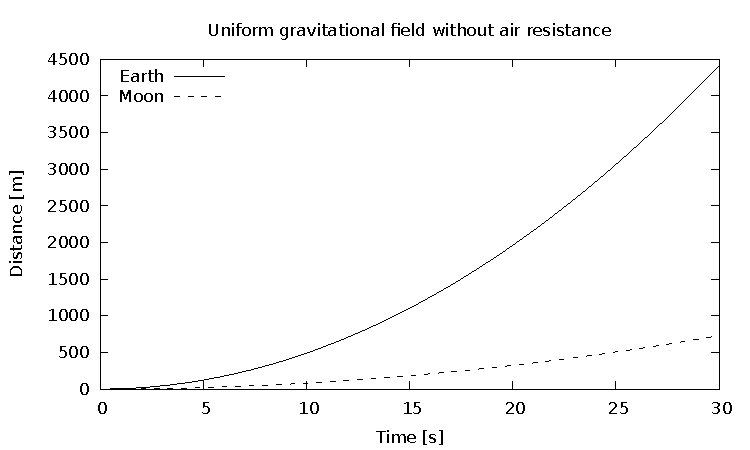
\includegraphics{gnuplot-bw}
 	\caption{Černobílá varianta obrázku generovaného programem Gnuplot}\label{fig:gnuplot-bw}
 \end{figure}
 
 \begin{figure}\centering
 	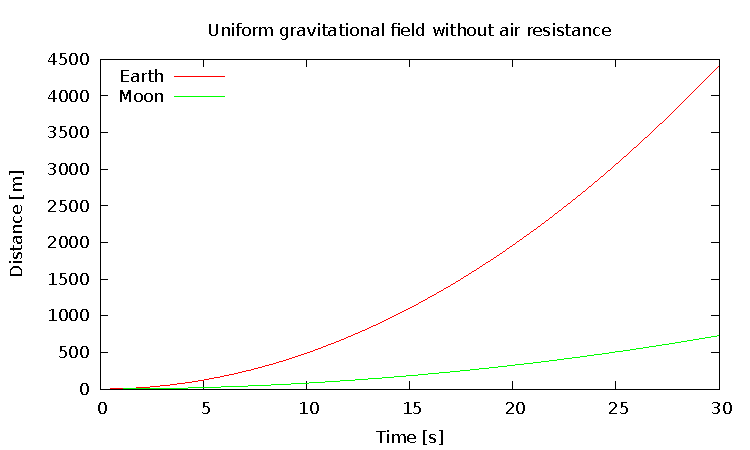
\includegraphics{gnuplot-col}
 	\caption{Barevná varianta obrázku generovaného programem Gnuplot}\label{fig:gnuplot-col}
 \end{figure}
 
 
 \subsection{Tabulky}
 
 Tabulky lze zadávat různě, např. v~prostředí \verb|tabular|, avšak pro jejich vkládání platí to samé, co pro obrázky -- použijte plovoucí prostředí, v~tomto případě \verb|table|. Například tabulka \ref{tab:matematika} byla vložena tímto způsobem.
 
 \begin{table}\centering
 	\caption[Příklad tabulky]{Zadávání matematiky}\label{tab:matematika}
 	\begin{tabular}{|l|l|c|c|}\hline
 		Typ		& Prostředí		& \LaTeX{}ovská zkratka	& \TeX{}ovská zkratka	\tabularnewline \hline \hline
 		Text		& \verb|math|		& \verb|\(...\)|	& \verb|$...$|		\tabularnewline \hline
 		Displayed	& \verb|displaymath|	& \verb|\[...\]|	& \verb|$$...$$|	\tabularnewline \hline
 	\end{tabular}
 \end{table}
 
% % % % % % % % % % % % % % % % % % % % % % % % % % % % 

\chapter{Obsah přiloženého CD}

\end{document}
